\section{Auswertung}
\label{sec:Auswertung}
Um die Gleichung \ref{eqn:} und \ref{eqn:} zu verifizieren sind die dafür Relevanten Messwerte in Tabelle \ref{tab:VdA} aufgetragen. Die Gegenstandsgröße $G$ des Pearl L beträgt $3.0 \cdot 10^{-2}$ m und die Vergrößerungen werden entsprechen $V_1 = \frac{b}{g}$ und $V_2 = \frac{B}{G}$ berechnet.
\begin{table}
  \centering
  \begin{tabular}{c c c c c c}
    \toprule
    $g / 10^{-2}$ m & $b / 10^{-2}$ m & $B / 10^{-3}$ m & $V_1$ & $V_2$ & $\left\lvert \frac{V_1 - V_2}{V_1} \right\rvert / \% $\\
   \midrule
    25	& 15.6	& 2.0 	& 0.62 & 0.66	& 6.6 	\\
    24	& 16.4	& 2.0	& 0.68 & 0.66	& 3.0	\\
    23	& 16.8	& 2.2	& 0.73 & 0.73	& 0.0	\\
    22	& 17.6	& 2.3	& 0.80 & 0.77	& 3.8	\\
    21	& 18.4	& 2.7	& 0.88 & 0.90	& 2.3	\\
    20	& 19.3	& 2.8	& 0.97 & 0.93	& 4.1	\\
    19	& 20.5	& 3.1	& 1.08 & 1.03	& 4.7	\\
    18	& 21.4	& 3.4	& 1.18 & 1.13	& 4.2	\\
    17	& 23.1	& 4.2	& 1.35 & 1.40	& 3.7	\\
    16	& 25.1	& 4.7	& 1.56 & 1.57	& 0.6	\\
    15	& 29.2	& 5.7	& 1.94 & 1.90	& 2.1	\\
    \bottomrule
  \end{tabular}
  \caption{Verifizierung des Abbildungsgesetzes}
  \label{tab:VdA}
\end{table}
Desweiteren wird zur ermittlung der Brennweite ein Plot erstellt,wonbei die Gegenstandsweiten auf die Y-Achse des Koordinatensystems aufgetragen werden und mit den entsprechenden Bildweiten, welche auf der X-Achse aufgetragen sind, verbunden. Aus dem Schnittpunkt der Graden lässt sich die Brennweite der Linse Ablesen. Aus Abbildung \ref{fig:} wird die Brennweite ?? abgelesen. 
\begin{figure}
  \centering
  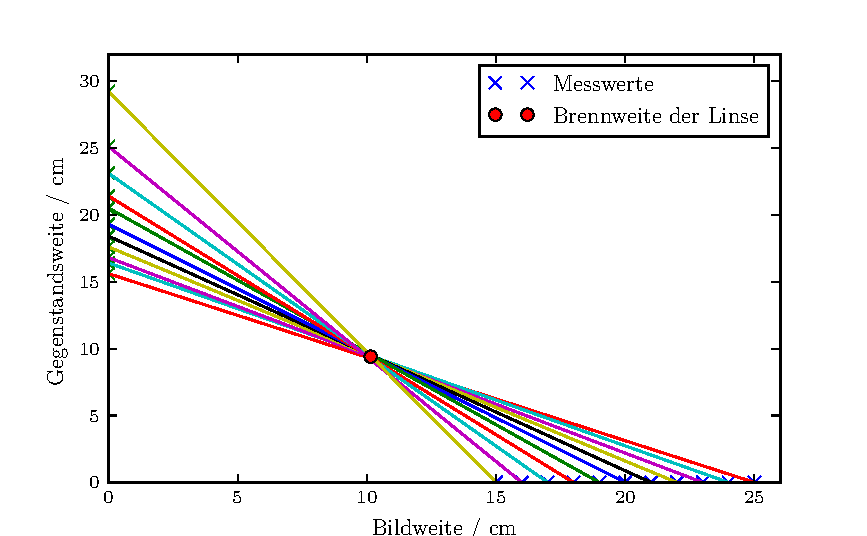
\includegraphics[height=5cm]{bekannt.pdf}
  \caption{<+caption text+>}
  \label{fig:<+label+>}
\end{figure}

\begin{figure}
  \centering
  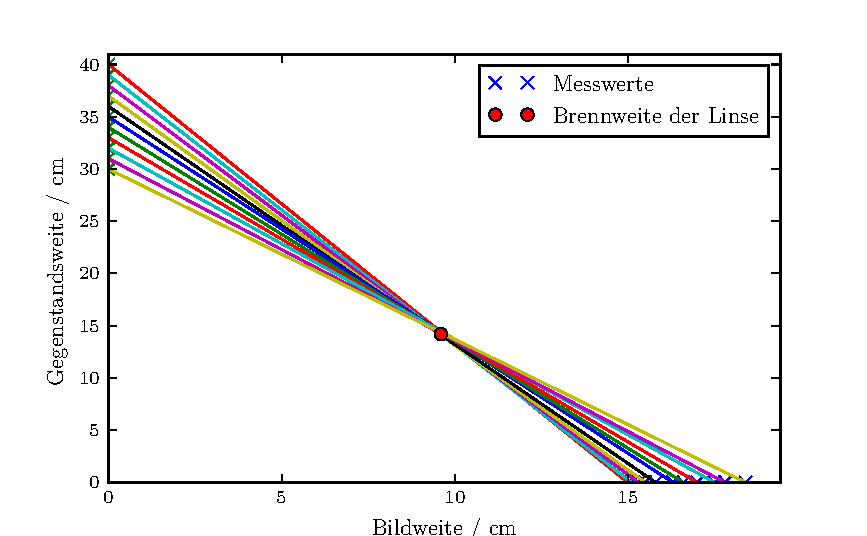
\includegraphics[height=5cm]{unbekannt.pdf}
  \caption{<+caption text+>}
  \label{fig:<+label+>}
\end{figure}

\begin{figure}
  \centering
    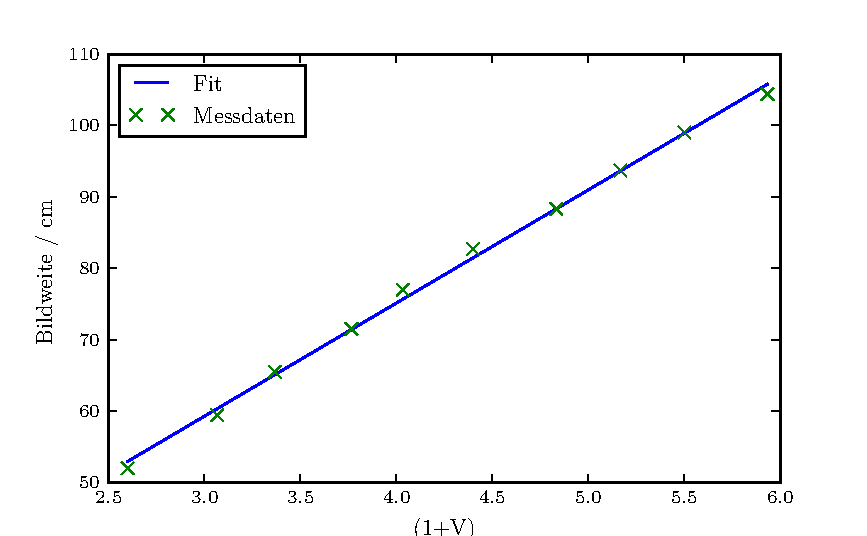
\includegraphics[height=5cm]{Abbe1.pdf}
  \caption{<+caption text+>}
  \label{fig:<+label+>}
\end{figure}

\begin{figure}
  \centering
  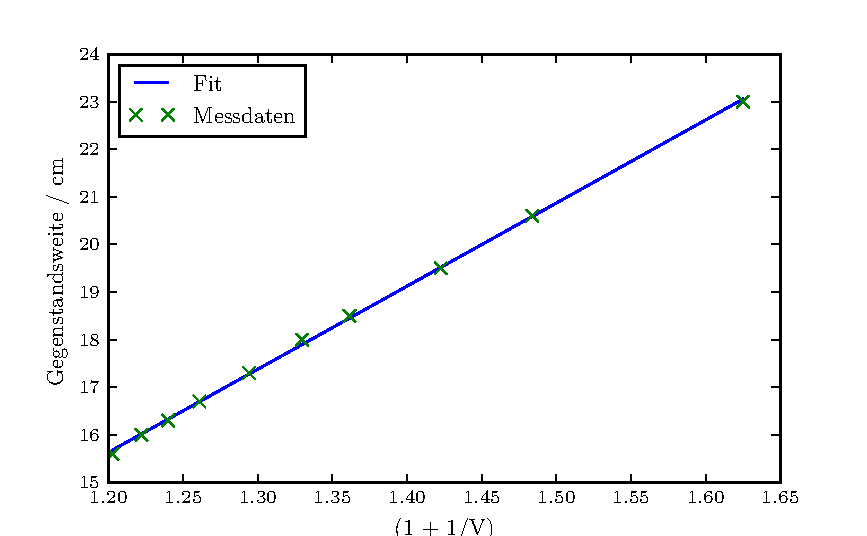
\includegraphics[height=5cm]{Abbe2.pdf}
  \caption{<+caption text+>}
  \label{fig:<+label+>}
\end{figure}
